\documentclass[11pt,fleqn]{exam}

\setlength {\topmargin} {-.15in}
\setlength {\textheight} {8.6in}
\usepackage{enumerate}
\usepackage{amsmath}
\usepackage{amssymb}
\usepackage{xcolor}
\usepackage[colorlinks = true,
            linkcolor = blue,
            urlcolor  = blue,
            citecolor = blue,
            anchorcolor = blue]{hyperref}
\usepackage{listings}
\usepackage{color} %red, green, blue, yellow, cyan, magenta, black, white
\usepackage{graphicx}
\definecolor{mygreen}{RGB}{28,172,0} % color values Red, Green, Blue
\definecolor{mylilas}{RGB}{170,55,241}
\newcommand{\nn}{~\newline \noindent }
\newcommand{\mname}[1]{\mbox{\sf #1}}
\usepackage{float}


\begin{document}

\lstset{language=Matlab,%
    %basicstyle=\color{red},
    breaklines=true,%
    morekeywords={matlab2tikz},
    keywordstyle=\color{blue},%
    morekeywords=[2]{1}, keywordstyle=[2]{\color{black}},
    identifierstyle=\color{black},%
    stringstyle=\color{mylilas},
    commentstyle=\color{mygreen},%
    showstringspaces=false,%without this there will be a symbol in the places where there is a space
    numbers=none,%
    numberstyle={\tiny \color{black}},% size of the numbers
    numbersep=9pt, % this defines how far the numbers are from the text
    emph=[1]{for,end,break},emphstyle=[1]\color{red}, %some words to emphasise
    %emph=[2]{word1,word2}, emphstyle=[2]{style},    
}
	
\begin{center}
	{\large \textbf{COMPSCI 4X03}}\\[2mm]
	{\huge \textbf{Assignment 3}}\\[6mm]
	{\large \textbf{Mingzhe Wang}}\\[2mm]
	{\large \textbf{McMaster University}}\\[6mm]
	{\large \today}
		
\end{center}
	
\medskip
		
\subsection*{Problem 1}
\begin{figure}[H]
  	\centering
  	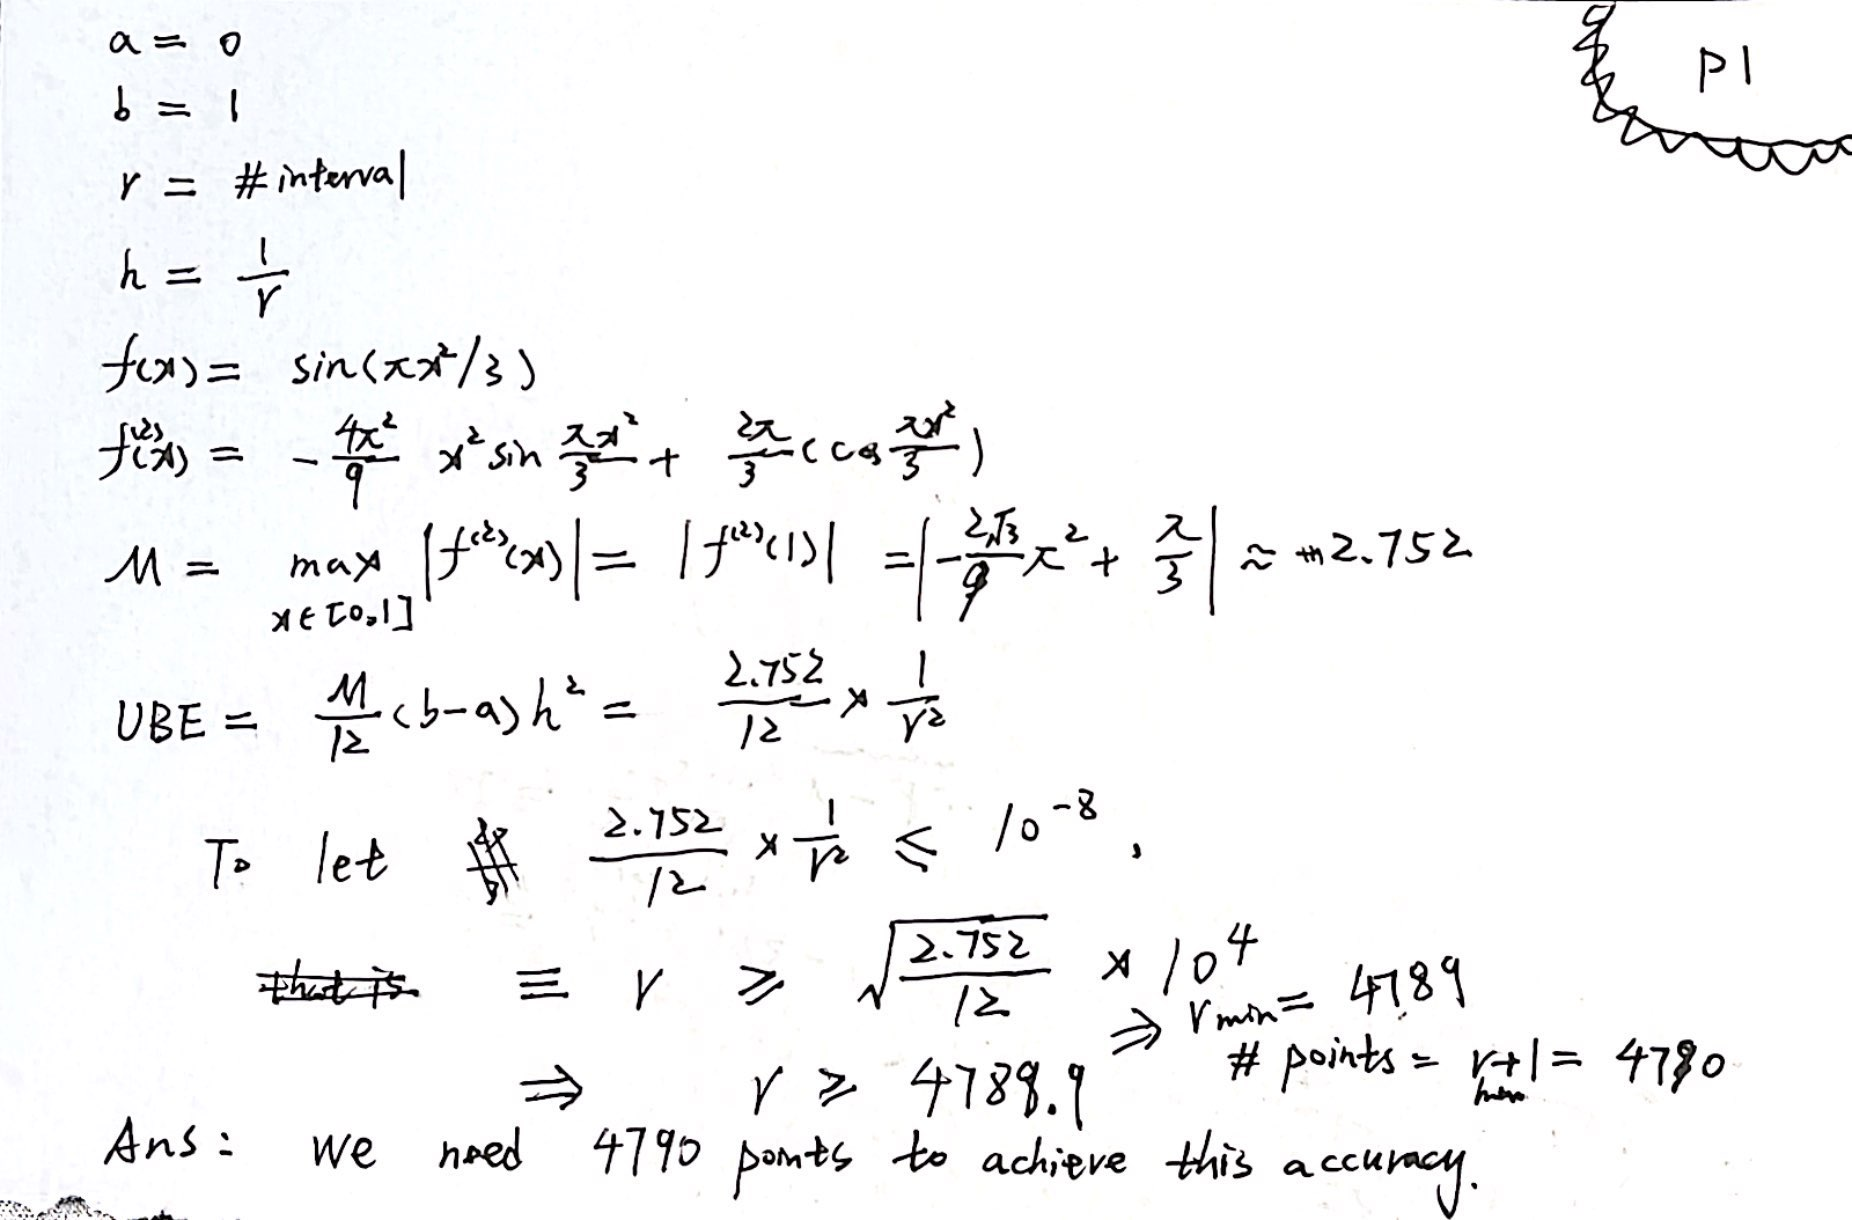
\includegraphics[width=1\textwidth]{p1.jpg}
\end{figure}

\subsection*{Problem 2}
\begin{figure}[H]
  	\centering
  	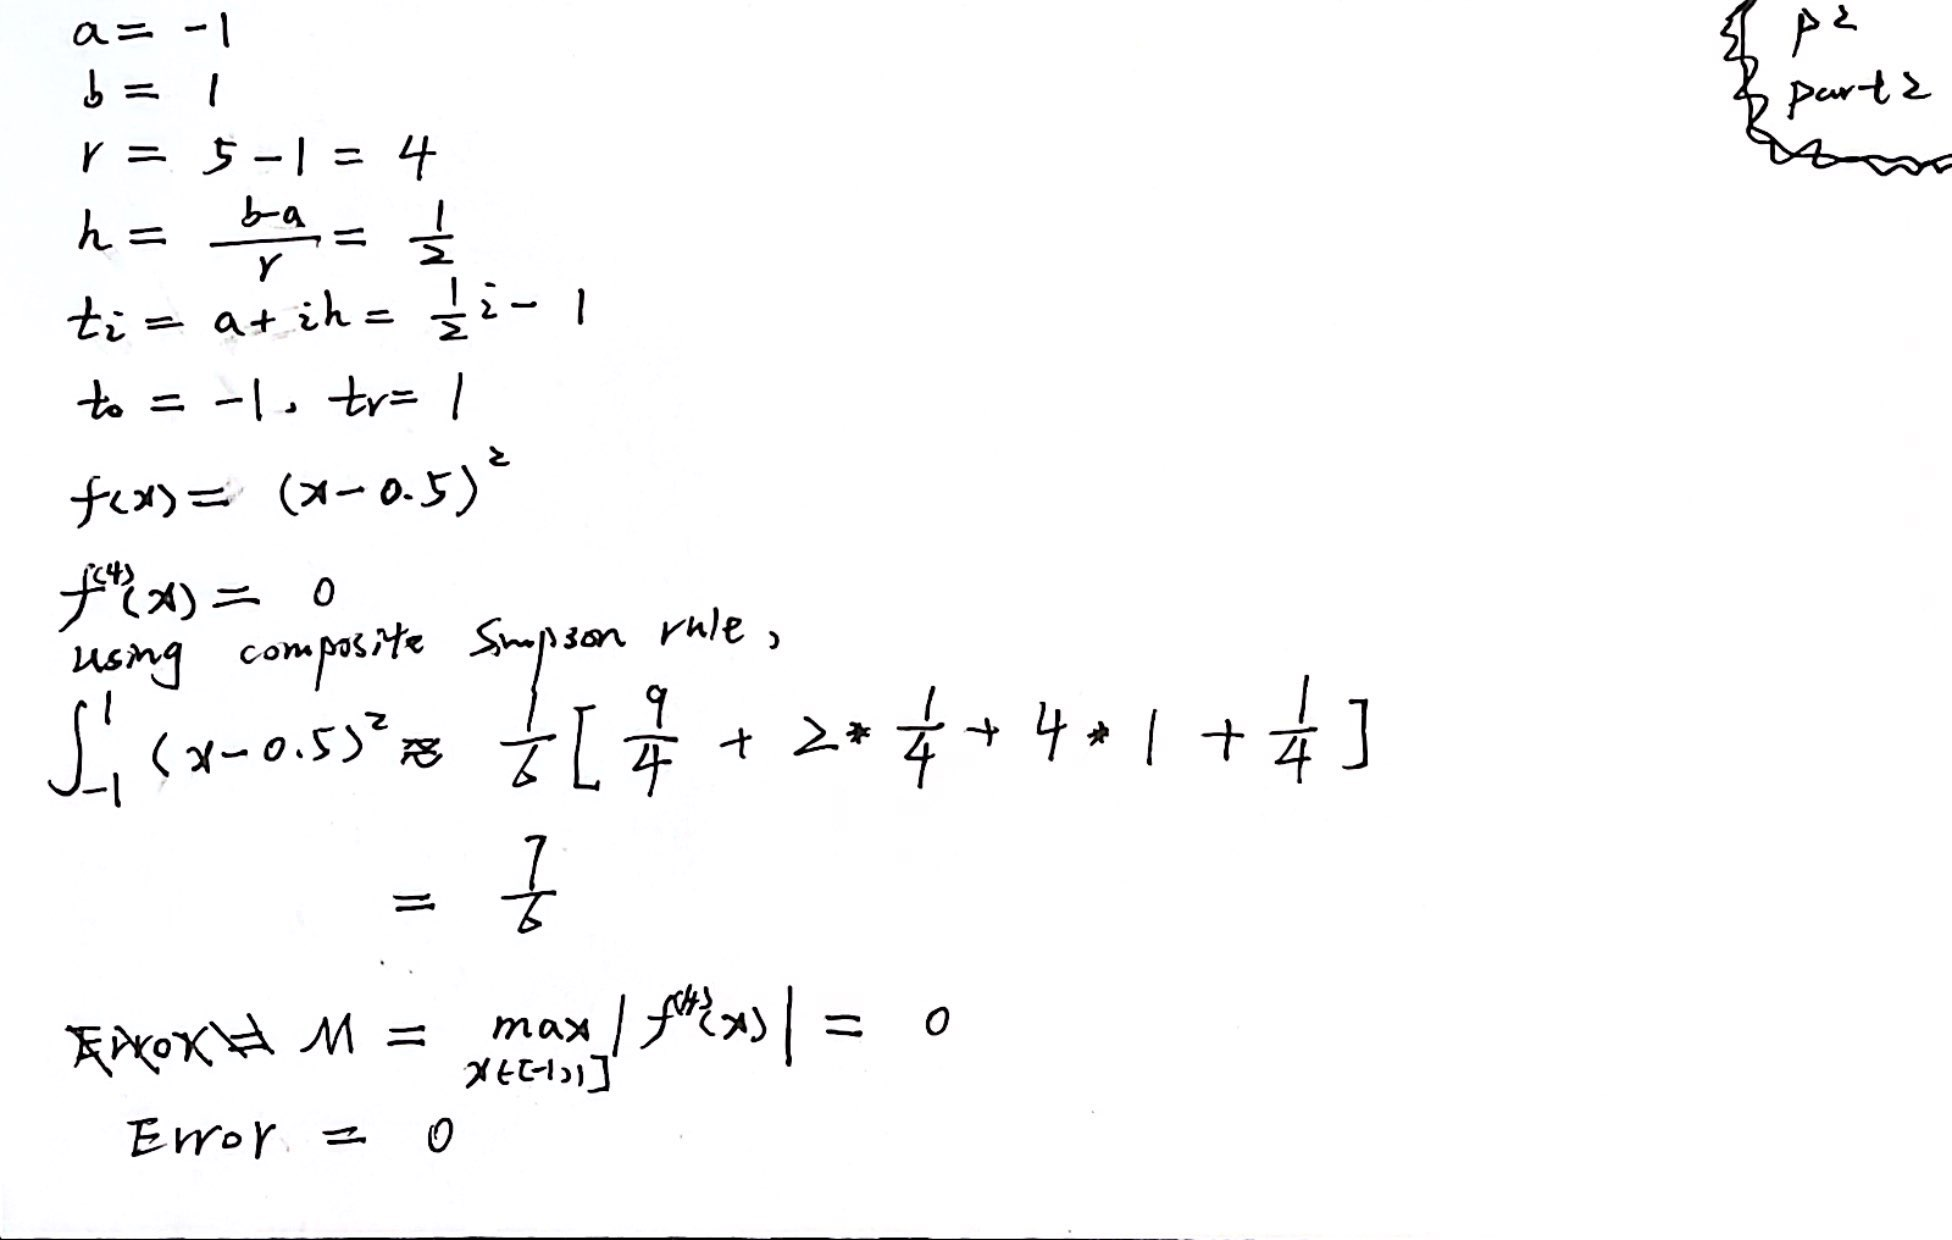
\includegraphics[width=1\textwidth]{p2.jpg}
\end{figure}

\subsection*{Problem 3}
\subsubsection*{Process}
\lstinputlisting{q3.m}
\subsubsection*{Output}
x1 = 2.960000\\
x2 = 1.746000\\
x3 = -1.460000\\
x4 = 1.314000\\
\subsubsection*{Compare}
The are similar but slightly different from direct measurement, because we also take into consideration the possible bias of only one reference value (we add more reference values for each x, so it could be more accurate).

\subsubsection*{Problem 4}
\subsubsection*{Function}
$$\int_{0}^{6\pi} sin^2(x) \,dx$$

\begin{figure}[H]
  	\centering
  	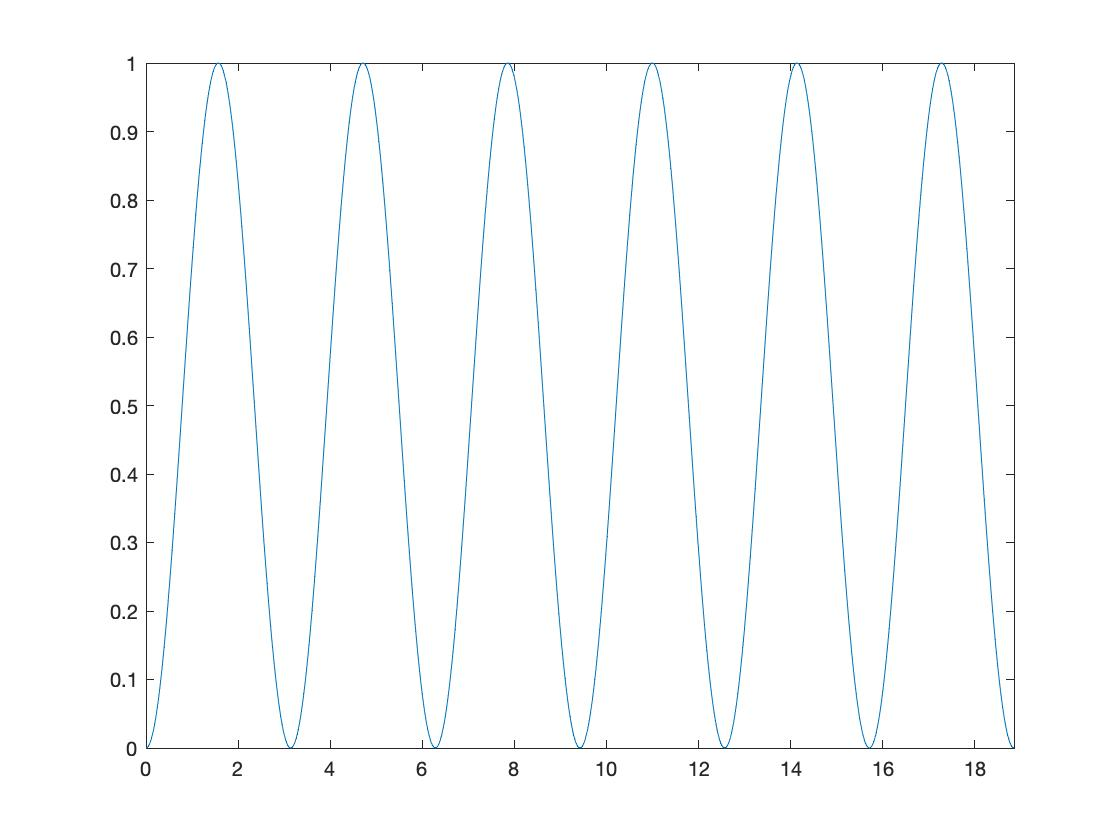
\includegraphics[width=1\textwidth]{p4.jpg}
\end{figure}

\begin{lstlisting}
composite Simpson error: 1.684973e-07
C1:       5703
adaptive Simpson error: 3.552714e-15
C2:         35
\end{lstlisting}

\subsubsection*{Problem 5}
\begin{figure}[H]
  	\centering
  	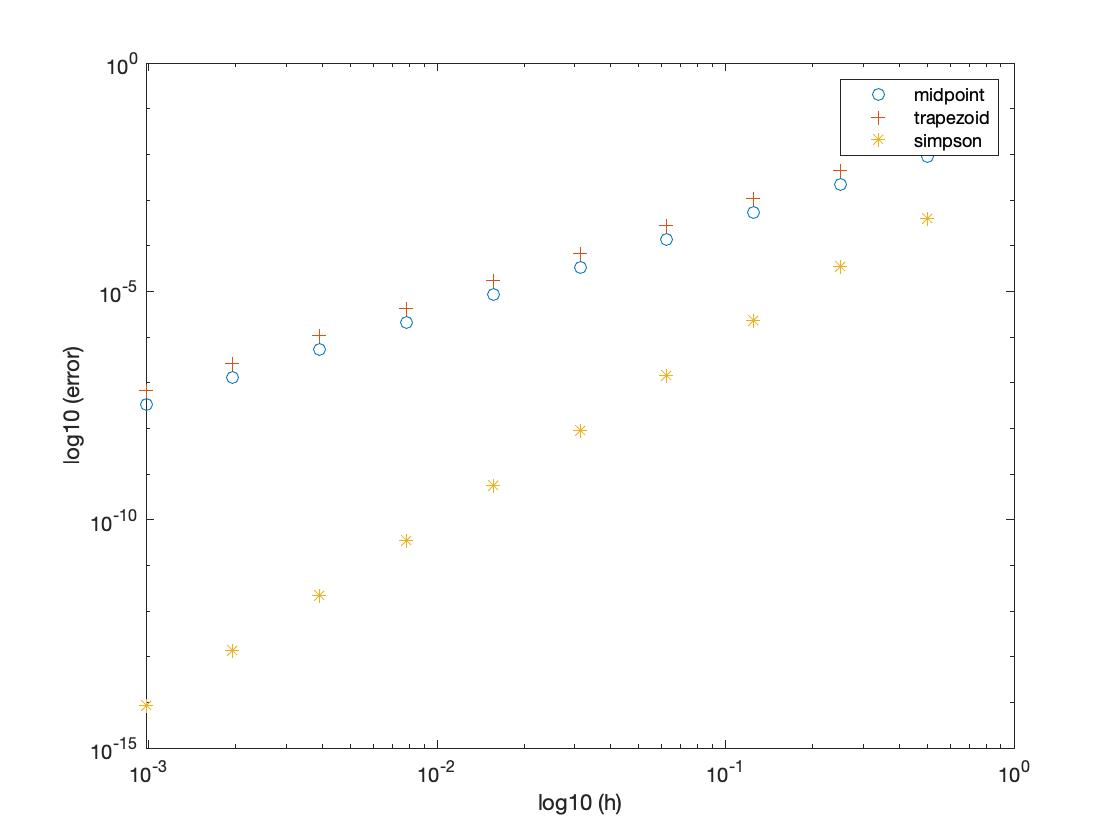
\includegraphics[width=1\textwidth]{p5.jpg}
\end{figure}

\noindent
\begin{lstlisting}
midpoint 3.48e-02*h^2.00
trapezoid 6.95e-02*h^2.00
simpson 7.87e-03*h^3.97
\end{lstlisting}


\subsubsection*{Problem 6}
\begin{lstlisting}
              a            b           c          d          e
Jupiter   -1.185397    0.022029   -0.495039   -0.145054   26.982216
Saturn    -1.166745    0.035963    0.116729   -1.089852   90.381602
Uranus    -1.194134    0.011627    1.827051   -0.259256  367.268144
Neptune   -1.167128    0.020704   -0.392687   -0.423158  903.808671
Pluto     -1.003337    0.238833   11.847098   12.717063  1290.679928
\end{lstlisting}

\end{document}


